\documentclass[sigconf]{acmart}


%---------------------
%	FIGURES
%---------------------
%\usepackage{graphicx}
%\graphicspath{{./images/}}

%---------------------
%	COLORS
%---------------------
%\definecolor{plt-blue}{HTML}{1f77b4}
%\definecolor{plt-orange}{HTML}{ff7f0e}

%---------------------
%	THEOREMS
%---------------------
\newtheorem{theorem}{Theorem}
\newtheorem{lemma}{Lemma}
\newtheorem{corollary}{Corollary}
\newtheorem{proposition}{Proposition}
\newtheorem{definition}{Definition}
\newtheorem{remark}{Remark}
\newtheorem{cost}{Cost function}
\newtheorem{model}{Model}
\newtheorem{assumption}{Assumption}



\usepackage{listings}

%-------------------------------
%	EXTRA CHARS AND SET NOTATIONS
%-------------------------------
% For sets (R and N) and eps files
\usepackage{upgreek}
\usepackage{bbm}			% mathbb vs mathds
\usepackage{xspace}

%---------------------
%	NEW COMMANDS
%---------------------

\newcommand{\ie}   			{i.e.\ }
\newcommand{\iid}   		{i.i.d.\ }
\newcommand{\eg}   			{e.g.\ }
\newcommand{\wrt}   		{w.r.t.\ }
\newcommand{\cdf}   		{c.d.f.\ }
%\newcommand{\st}   			{\mbox{s.t.\ }}
\newcommand{\as}   			{\mbox{~a.s.}}
\newcommand{\aas}   		{\mbox{~a.a.s.}}


\newcommand{\norm}[1]{\left\lVert#1\right\rVert}
\newcommand{\normh}[1]{\left\lVert#1\right\rVert_{\HH}}
\newcommand{\p}{\partial} %Partial
\newcommand{\dd}{\mathrm{d}} % d droit
\newcommand{\XX}{\mathcal{X}}
\newcommand{\AAA}{\mathcal{A}}
\newcommand{\BB}{\mathcal{B}}
\newcommand{\HH}{\mathcal{H}}
\newcommand{\DD}{\mathcal{D}}
\newcommand{\bigo}{\mathcal{O}}
\newcommand{\sca}[2]{\left \langle #1 \middle| #2 \right \rangle} % inner product
\newcommand{\pa}[1]{\lfloor #1 \rfloor} % partie entière
\newcommand{\var}{\mathrm{Var}} % variance
\newcommand{\RR}{\mathbb{R}} % espace réel
\newcommand{\CC}{\mathbb{C}} % espace complexe
\newcommand{\PP}{\mathbb{P}} % mesure de probabilité P
\newcommand{\QQ}{\mathbb{Q}} % mesure de probabilité Q
\newcommand{\EE}{\mathbb{E}} % espérance E
\newcommand{\ZZ}{\mathbb{Z}} % mesure de probabilité Z
\newcommand{\NN}{\mathbb{N}} % entiers positifs
\newcommand{\GG}{\mathcal{G}} % graph
%\newcommand\intervalint[1]{\llbracket #1 \rrbracket} % produit scalaire
\newcommand\red[1]{\textcolor{red}{#1}} % colorer en rouge
\newcommand\gray[1]{\textcolor{gray}{#1}} % colorer en gris
\newcommand{\PPP}{\mathcal{P}} % ensemble des partitions
\newcommand{\SSS}{\mathcal{S}} % ensemble des partitions
\newcommand\intervalint[1]{[\![ #1 ]\!]} % intervalle entier
\newcommand\und[1]{\underline{#1}} % quick underline
\newcommand\sta[1]{#1^{\star}} % quick star
\newcommand\one{\mathds{1}} % indicatrice
% \newcommand\hatt[1]{\hat{#1}} % quick star
\DeclareMathOperator*{\argmax}{\mbox{arg max}} % arg max qui marche mieux
\DeclareMathOperator*{\argmin}{\mbox{arg min}} % arg max qui marche mieux
%\newcommand\res[2]{#1\ (\pm #2)} % pour les resultats: m (+- std)
%\newcommand\code[1]{\fcolorbox{white}{gray!15}{\color[rgb]{0,.3,.6}\textsf{#1}}}
%\newcommand\ruptures{\code{ruptures}} % package ruptures
%\newcommand{\pp}{\mathbf{p}} %partition
% \newcommand{\ttt}{\mathbf{t}} %change points
%\newcommand{\ttt}{\mathcal{T}} %change points
% checkmark and x mark
%\newcommand{\cmark}{\ding{51}}%
%\newcommand{\xmark}{\ding{55}}%
% unfilled star (starw(hite))
%\newcommand{\starw}{\ding{73}}%
% filled star (starb(lack))
%\newcommand{\starb}{\ding{72}}%
%\DeclareMathOperator{\tr}{tr} % trace operator
%\DeclareMathOperator{\diag}{diag} % trace operator


% complex i
\newcommand{\iu}{{i\mkern1mu}}
\usepackage{subcaption}

%%
%% \BibTeX command to typeset BibTeX logo in the docs
\AtBeginDocument{%
  \providecommand\BibTeX{{%
    Bib\TeX}}}



\setcopyright{acmcopyright}
\copyrightyear{2023}
\acmYear{2023}
% \acmDOI{XXXXXXX.XXXXXXX}

%% These commands are for a PROCEEDINGS abstract or paper.
\acmConference[MVA 2023]{MVA 2023}{December
  2023}{Paris, FR}

% \acmPrice{15.00}
% \acmISBN{978-1-4503-XXXX-X/18/06}


\begin{document}

%%
%% TITLE
\title{Review of Spectral Graph Convolutions for Population-based Disease Prediction}

%%
%% AUTHORS
\author{Manal Akhannous}
\affiliation{%
  \institution{ENPC}
  \streetaddress{Cité Descartes, 8 Av Blaise Pascal}
  \city{Champs-sur-Marne}
  \country{France}
}
\email{manal.akhannous@eleves.enpc.fr}

\author{Ines Vati}
\affiliation{%
  \institution{ENPC}
  \streetaddress{Cité Descartes, 8 Av Blaise Pascal 6 et}
  \city{Champs-sur-Marne}
  \country{France}
}
\email{ines.vati@eleves.enpc.fr}

\author{Balthazar Neveu}
\affiliation{%
  \institution{ENS Paris-Saclay}
  \city{Saclay}
  \country{France}
}
\email{balthazar.neveu@ens-paris-saclay.fr}


\renewcommand{\shortauthors}{MVA et al.}

%% ABSTRACT
\begin{abstract}
  We'll review the paper Spectral Graph Convolutions for Population-based Disease Prediction \cite{Parisot17}

\end{abstract}


%%
%% Keywords. The author(s) should pick words that accurately describe
%% the work being presented. Separate the keywords with commas.
\keywords{Graph, Spectral, Convolution, Medical, Disease}


\received{10 December 2023}
\received[revised]{10 December 2023}
\received[accepted]{10 December 2023}

%% TITLE
\maketitle


\section{Introduction}

%(context problematique médicale, target application (disease prediction) low data regim, intérêt d'avoir des graphs , Parisot idée d'utiliser des graphs applique Kipf )

\quad In recent years, the intersection of machine learning and medical research has seen an increase in innovative approaches to analyze complex patterns in population health data. One such approach is presented in the paper "Spectral Graph Convolutions for Population-based Disease Prediction," which introduces the use of Graph Convolutional Networks (GCN) for analyzing brain-related disorders in populations. By utilizing a graph structure that combines imaging and non-imaging data, this paper makes significant advancements in disease prediction.

The paper addresses the challenges posed by the growing dimensionality of health datasets and the limited availability of labeled instances. By representing populations as graphs, with each subject as a vertex and edges encoding phenotypic information, the authors propose a methodology that leverages auxiliary information to improve disease prediction. The graph structure captures the similarities between subjects, providing a nuanced representation of the population.

The Graph Convolutional Network (GCN) model is trained on partially labeled graphs, enabling it to predict classes for unlabeled nodes based on node features and pairwise associations between subjects. This novel use of graph structures demonstrates improved accuracy in disease prediction compared to traditional linear classifiers. The application of GCN is tested on different databases, showing promising results in brain-related disorders.

The proposed method has applications in various domains of medical research, with a primary focus on disease prediction. Its effectiveness is demonstrated by predicting disease conversion, particularly the transition from Mild Cognitive Impairment (MCI) to Alzheimer's Disease (AD) in the ADNI database. The GCN model exhibits promising accuracy in disease prediction compared to linear classifiers, highlighting its potential clinical relevance.

In addition to disease prediction, the paper addresses a critical issue in medical diagnosis: the reliance on behavioral tests for identifying conditions such as Autism Spectrum Disorder (ASD) or Alzheimer's. Many related diseases are often diagnosed only through subjective observations and behavioral assessments, leading to delayed identification and intervention.

The impact of introducing a new diagnostic tool, such as the GCN-based methodology proposed in the paper, is profound. Early diagnosis enabled by this model offers a transformative opportunity for patients. It allows for timely access to medical treatments and interventions, potentially slowing down disease progression and improving overall outcomes. The ability to identify and predict diseases at earlier stages not only enhances patient care but also opens avenues for targeted therapies and interventions tailored to individual needs.

Furthermore, the model's capacity to integrate various data types into a unified graph structure enables a more comprehensive understanding of the diseases under consideration. Moreover, graph-based methods have an interpretability advantage over traditional deep learning Multi-Layer Perceptrons (MLP). The graph structure inherently captures relationships between subjects, providing a transparent and interpretable framework for understanding the model's decision-making process. This interpretability is crucial in the medical domain, where clinicians and researchers need to trust and comprehend the models' predictions for effective integration into clinical practice.

In summary, the paper introduces an advanced methodology for population-based disease prediction, offering a promising solution to the challenges posed by traditional diagnostic methods. The incorporation of graph-based models not only enhances prediction accuracy but also holds the potential to revolutionize the landscape of early disease diagnosis and intervention, ultimately improving patient outcomes.
\section{Related Work}

other methods 

what manal has started to do

\section{Proposed method}

\subsection{Graph construction} 


Autism spectrum disorder (ASD) is now recognized to occur in more than 1\% of children. Despite continuing research advances, their pace and clinical impact have not kept up with the urgency to identify ways of determining the diagnosis at earlier ages, selecting optimal treatments, and predicting outcomes. The researchers \cite{Parisot17} proposed to tackle those challenges and applied their method on the Autism Brain Imaging Data Exchange (ABIDE) dataset, which consists of highly heterogeneous functional MRI data acquired at multiple sites. Resting-state functional magnetic resonance imaging (rs-fMRI) is a neuroimaging technique that measures and analyses brain activity in a resting state, i.e., when a person is not engaged in any specific task. 
It is based on the principle that different regions of the brain exhibit correlated spontaneous fluctuations in blood oxygen level-dependent (BOLD) signals even in the absence of an explicit stimulus or task. These fluctuations are thought to reflect the intrinsic functional connectivity of the brain. 

The authors \cite{Parisot17} proposed to construct a population graph integrating imaging and non-imaging data. 
They defined the feature vector $x(v)$ of each patient $v$ as the vectorized form $X_{v}$ of its functional connectivity matrix. Connectivity matrices represent the strength of functional connections between different brain regions for a given subject. They are derived from rs-fMRI data by computing the Pearson's correlation coefficient between brain regions' activity patterns, offering a concise representation of interregional communication within brain regions. The figure \ref{fig:connectivity_matrix} display the connectivity matrix obtained for three patients in the ABIDE dataset. \blue{Note that they also applied the Fisher transform of the Pearson correlation but we did not do it}.  

\begin{figure*}[h!]
    \begin{subfigure}{0.3\textwidth}
        \centering
        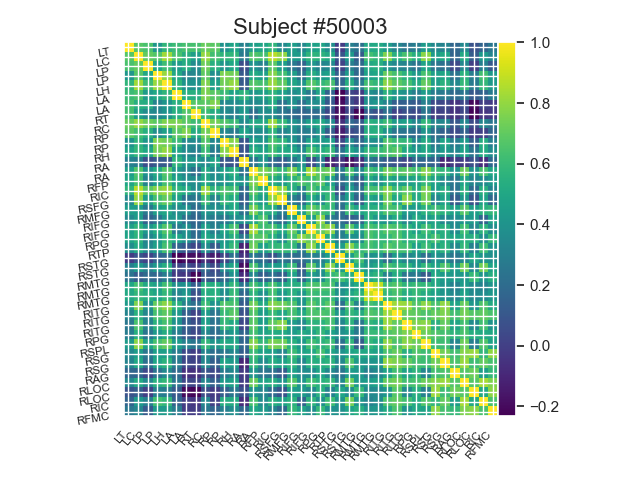
\includegraphics[width=\textwidth]{figures/ex_connectivity_matrix_pitt_ASD.png}
        \caption{\centering Patient with ASD in PITT acquisition site} 
        \Description{}
    \end{subfigure}
    \hfill
    \begin{subfigure}{0.3\textwidth}
        \centering
        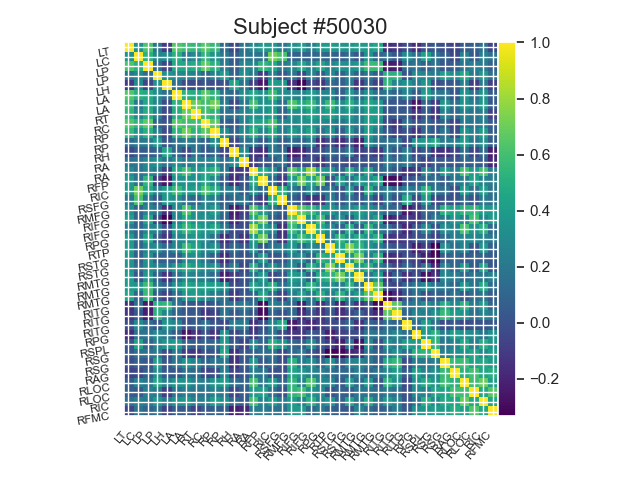
\includegraphics[width=\textwidth]{figures/ex_connectivity_matrix_pitt_H.png}
        \caption{\centering Patient without ASD in PITT acquisition site} 
        \Description{}
    \end{subfigure}
    \hfill
    \begin{subfigure}{0.3\textwidth}
        \centering
        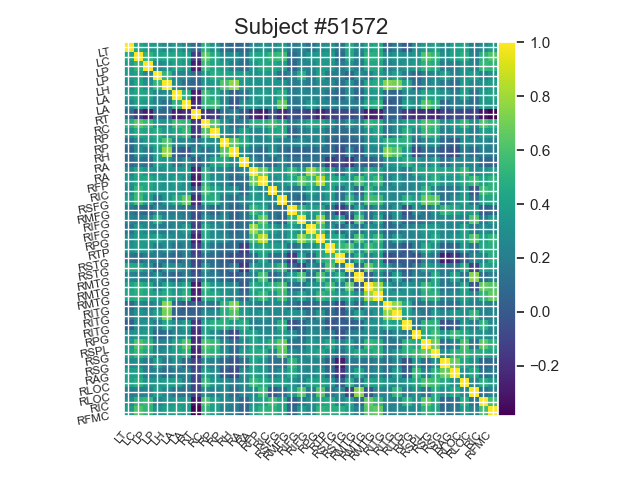
\includegraphics[width=\textwidth]{figures/ex_connectivity_matrix_sbl_ASD.png}
        \caption{\centering Patient with ASD in SBL acquisition site \qquad }
        \Description{}
    \end{subfigure}
    \caption{Connectivity matrix of given subjects. Each brain region is indicated in the x-axis and y-axis. The colour of the pixel indicates the strength of the functional connection between the two regions. We did not plot all 111 regions for the sake of readability.}
    \Description{}
    \label{fig:connectivity_matrix}
\end{figure*}

The connectome encapsulates the intricate web of connections between different brain regions. In figure \ref{fig:connectome}, we depict the brain graph associated with the connectivity matrix computed in figure \ref{fig:connectivity_matrix}. The coordinate of brain regions are derived from the Harvard-Oxford atlas\footnote{http://preprocessed-connectomes-project.org/abide/Pipelines.html} which defines a mask containing 111 regions of interest (ROIs).

\begin{figure}[h!]
    \centering
    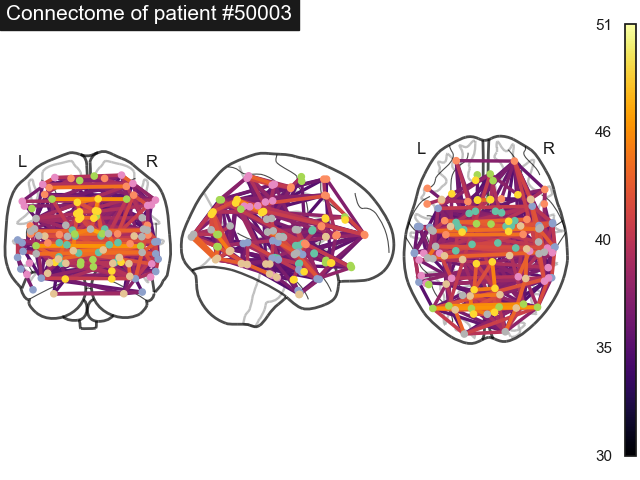
\includegraphics[width=0.45\textwidth]{figures/ex_connectivity_pitt_ASD.png}
    \caption{Connectome graph of a given patient. Each node represents a specific brain region and edges correspond to the connectivity between two regions as plotted in figure \ref{fig:connectivity_matrix}. This representation offers a unique insight into the patient's neural architecture, highlighting the potential correlates of cognitive processes, as well as providing valuable information for understanding the impact of neurological conditions. Note that the exact values of the edges weights were multiplied by 50 to improve the readability of the figure.}
    \Description{}
    \label{fig:connectome}
\end{figure}

Given the matrix's high dimensionality (number of patients $\times 6217$), the authors employed a ridge classifier to identify the most discriminative features within the training set.

They modelled the interactions between individuals via the definition of the graph edges, $\EE$ which writes as follows for two nodes $v$ and $v'$ :
$$ 
    \WW(v, v') = Sim(X_v, X_{v'}) \left[\delta_{M_{SEX}(v)}(M_{SEX}(v')) + \delta_{M_{SITE}(v)}(M_{SITE}(v')) \right]
$$

$\delta$ is the Kronecker delta function.  $M_{SITE}$ and $M_{SEX}$ are contextual information. $Sim$ is a similarity measure between the connectivity matrices of the subjects $v$ and $v'$. In \cite{Parisot17}, the authors used the correlation distance 
$$
Sim(X_v, X_{v'}) =  1 - \frac{(X_v - \widebar{X}_v).(X_{v'} - \widebar{X}_{v'})}{\norm{X_v -\widebar{X}_{v}}_2\norm{X_{v'} - \widebar{X}_{v'}}_2}
$$
where $\widebar{X}_v$ is the mean of the elements of the vectorized connectivity matrix of the patient $v$. 

On the figure \ref{fig:sorted_adjacency}, certain sets or squares stand out with significantly higher correlation along the diagonal, demonstrating the similarity between this metadata information. 

\begin{figure}[h!]
    \centering
    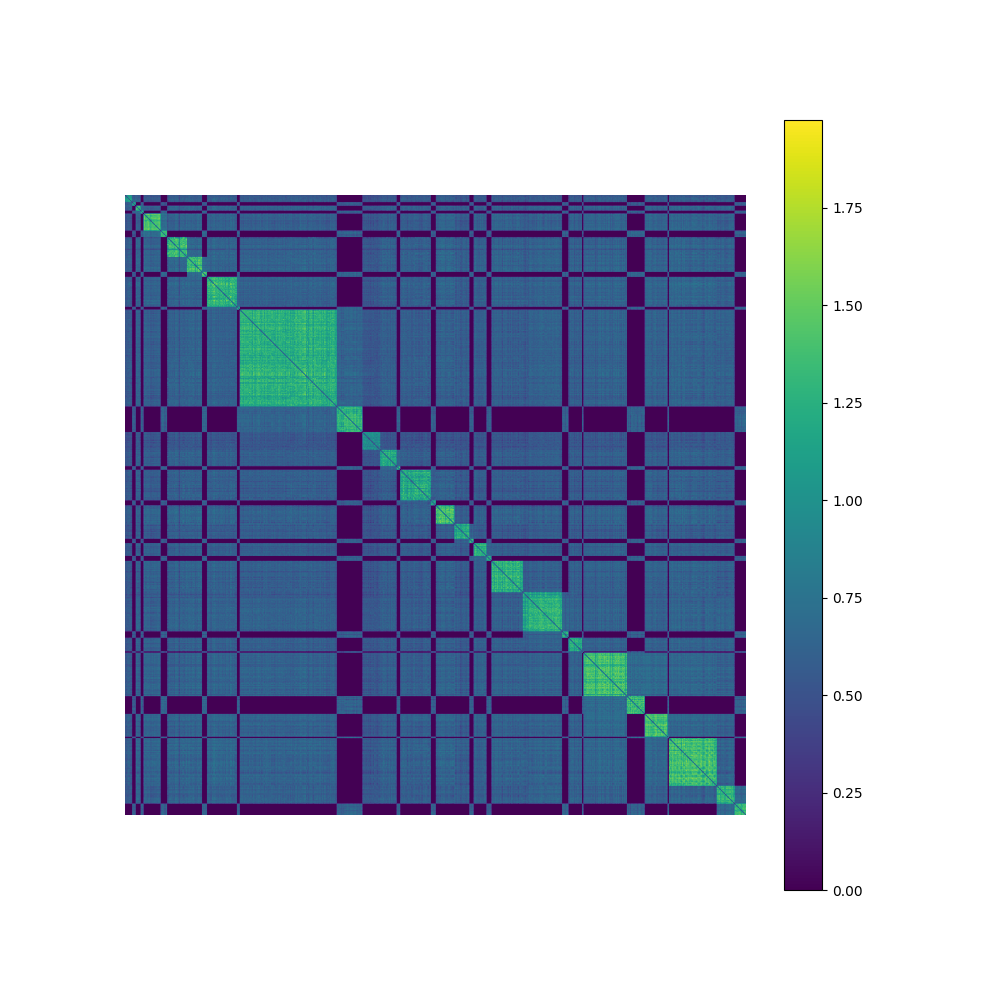
\includegraphics[width=0.45\textwidth]{figures/sorted_adjacency_by_site_id_by_sex.png}
    \caption{Edge weights sorted by \textit{acquisition sites} and \textit{gender}. This plot explains the process of using contextual and phenotypic information to construct connections in the graph. The fundamental concept underlying this graph structure is to exploit site information, anticipating greater comparability among subjects within the same site owing to diverse acquisition protocols.}
    \Description{}
    \label{fig:sorted_adjacency}
\end{figure}

To classify from this brain population graph, the authors \cite{Parisot17} proposed to use a Graph Convolutional Neural Network (GCN) on graphs. We will now present the mathematical framework of these networks.

\subsection{Mathematical framework on Graph Spectral Theory}
\subsubsection{The main challenges of signal processing on graphs} 

The generic data representation forms of graphs are useful for describing the geometric structures of data domains in very different application fields.
However, classical tools and techniques from signal processing can not be used seamlessly on graphs, unlike audio signal and images \cite{shuman_emerging_2013}.

In particular, graphs have no inherent ordering of the vertices, unlike images where each pixel is uniquely identified by its position within the image. We therefore need algorithms that are node-order equivariant: they should not depend on the ordering of the nodes \cite{daigavane_understanding_2021}. We may also need localized transforms that compute information about the data at each vertex by using data from a small neighbourhood of vertices close to it in the graph.

Graphs can also be very large but, in our study, we consider sparse population graphs, \ie individuals or nodes are connected to a limited number of nodes \footnote{We also say that the number of edges is linear in the number of nodes.}.
Spectral graph theory has enabled constructing, analysing, and manipulating graphs.

%In signal processing on graphs, it is leveraged as a tool to define frequency spectra and expansion bases for graph Fourier transforms.

In this section, we present some basic definitions from spectral graph theory that will be needed to apply neural networks on graphs. As stated previously, we consider an undirected, connected, weighted graph $\mathcal{G} = \{\mathcal{V}, \EE, \WW\}$. 

\subsubsection{The non-normalized and normalized Graph Laplacian}

The non-normalized graph Laplacian, also called the combinatorial graph Laplacian, is defined 
as $\mathbf{L} = \mathbf{D}-\mathbf{W}$, where the degree matrix $\mathbf{D}$ 
is a diagonal matrix 
whose $i$th diagonal element, $d_i$, is equal to the sum of the weights of all edges incident to the vertex $i$
(e.g. the sum over the rows of $\WW$).
%The graph Laplacian is a difference operator defined for any signal $f$, as follows :
%$$
%(\mathbf{L}f)(i) = \sum_{j\in\mathcal{N}_i} W_{i, j}[f(i) - f(j)]
%$$
%where $\mathcal{N}_i$ is the set of vertices connected to vertex $i$ by an edge.

The graph Laplacian $\mathbf{L}$ is a real symmetric matrix, it has therefore real, non-negative eigenvalues $\{\lambda_l\}_{l=0, \dots, N-1}$. 
We denote their associated  orthonormal eigenvectors by $\{u_l\}_{l=0,\dots, N-1}$. In the following, $\Lambda$ and $U$ denote the diagonal matrix of eigenvalues and the matrix of eigenvectors, respectively.

Since we consider connected graphs, the eigenvalue $\lambda_0=0$ has multiplicity $1$  \cite{shuman_emerging_2013}. 
%\textit{(There are as many null eigen values as there are connected components in the graph.)}

A popular practice is to normalize each weight $W_{i, j}$ by a factor of $\frac{1}{\sqrt{d_id_j}}$.
Doing so leads to the normalized graph Laplacian, which is defined as $\widetilde{\mathbf{L}} = D^{-1/2}\mathbf{L}D^{-1/2} = I_N - D^{-1/2}\mathbf{W}D^{-1/2}$. This strategy is used to improve the stability of gradient flow during backpropagation in neural networks. This can be valuable in mitigating the vanishing gradient problem and facilitating the training of deeper and more expressive models on graph data.


\subsubsection{A Graph Fourier Transform and Notion of Frequency}
The Fourier transform for an analogous function $f$
$$
\hat{f}(\xi) = \sca{f}{e^{2\pi i\xi t}} = \int_{\RR} f(t)e^{-2\pi i \xi t}dt
$$
is the expansion of a function $f$ in terms of the complex exponentials, which are the eigenfunctions of the one-dimensional Laplace operator $\Delta$ :
$$
-\Delta (e^{2\pi i \xi t}) = -\frac{\partial^2}{\partial t^2} e^{2\pi i \xi t} = (2\pi i\xi)^2 e^{2\pi i \xi t}
$$
Similarly, we can define the \textit{Graph Fourier Transform} $\hat{f}$ of any function on the vertices of $\GG$ as the expansion of $f$ in terms of the eigenvectors of the graph Laplacian $\hat{f}(\lambda_l) = \sca{f}{u_l} = \sum_{i=1}^{N} f(i)u_l^*(i)$ : 
where $u_l^*(i)$ is the conjugate of $u_l(i)$ : 
\begin{equation}
    \hat{f} = U^Tf
\end{equation}

The \textit{inverse graph Fourier transform} is then given by $f(i) = \sum_{i=1}^{N} \hat{f}(\lambda_i)u_l(i)$ : 
\begin{equation}
    f = U\hat{f}
\end{equation}

Note that, in our case, the signal $f:\mathcal{V}\rightarrow\RR^N$ associates a feature vector to each node of the graph.

\subsubsection{Spectral Graph Convolutions}

Spectral convolution of the signal $f$ with a filter $g_\theta$ is defined as $g_\theta * f = g_\theta(\widetilde{\mathbf{L}})f = Ug_\theta(\Lambda)U^Tf = U g_\theta(\Lambda)\hat{f}$. 
Indeed, we recover the property that the convolution in the vertex domain is equivalent to a multiplication in the graph spectral domain.

Polynomial filters, defined as $g_\theta(\Lambda) = \sum_{k=0}^{K-1}\theta_k\Lambda^k$, are commonly used in localized convolutions. Those filters are localized thanks to the lemma 5.2 in \cite{hammond_wavelets_2011}. We can show that for some integer $s$ and for any 
vertices $m$ and $n$ in the graph $\GG$, if $d_\GG(m, n) > s$ then $(L^s)_{m, n} = 0$. $d_\GG(m, n)$ denotes the number of edges in the shortest path connecting the nodes $m$ and $n$.
It follows that a $K$-order polynomial filter is strictly $K$-localized, \ie it only depends on the $K$-hop neighbourhood of each vertex. In the studied paper \cite{Parisot17}, the authors chose $K=3$.\\ 
Furthermore, according to the lemma \ref{lemma:chebyDecomposition}, such filters can be well approximated by a truncated Chebyshev expansion of the form $g_\theta(\widetilde{\mathbf{L}}) = \sum_{k=0}^{K-1}\theta_kT_k(\widetilde{\mathbf{L}})$ where $T_k$ is the $k$th Chebyshev polynomial of the first kind.
\begin{lemma}\label{lemma:chebyDecomposition}
    In the appropriate Sobolev space, the set of Chebyshev polynomials form an orthonormal basis, so that a function in the same space can, on $-1\leq x \leq 1$, be expressed via the expansion : $$g(x) = \sum_{n=0}^{\infty} a_nT_n(x)$$.
\end{lemma}
This decomposition significantly reduces the computational complexity of the convolution operator \cite{Parisot17}.

%polynomials of Laplacian of degree $d$ : the node $v$ is convolved with nodes that are at most at a distance $d$. Thus, these polynomials filters are localized.

\subsubsection{A simple illustration}

We have implemented a simple application of the spectral graph convolution on a toy graph. 
On the illustration \ref{fig:toyGraph}, we notice that the greater the order of the convolution,  the more the signal is smoothed, and the less the graph Laplacian have null coefficients.

 \begin{figure}
    \centering
    \begin{subfigure}{0.45\textwidth}
        \centering
        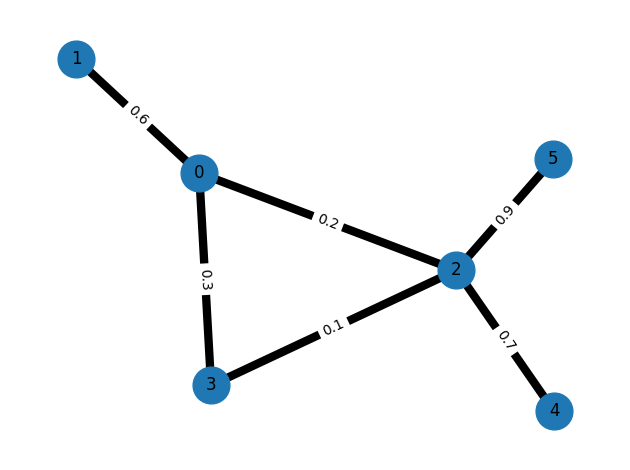
\includegraphics[width=0.45\textwidth]{figures/toy_graph_init.png}
        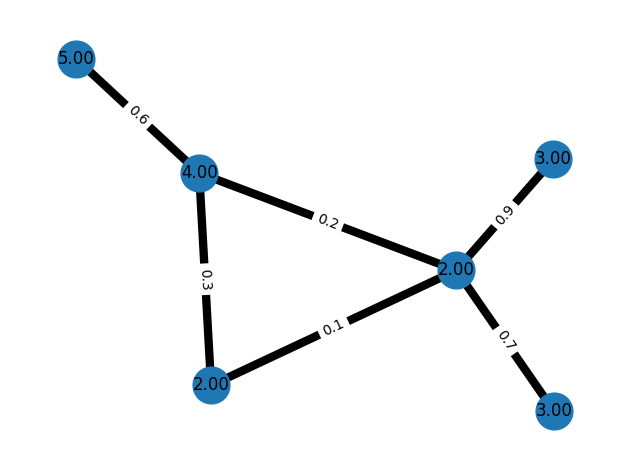
\includegraphics[width=0.45\textwidth]{figures/toy_graph_conv_K1.png}
        \caption{Toy graph\\ $\leftarrow$ indexes of the nodes | initial features values ($K=1$) $\rightarrow$}
    \end{subfigure}
    \hfill
    \begin{subfigure}{0.45\textwidth}
        \centering
        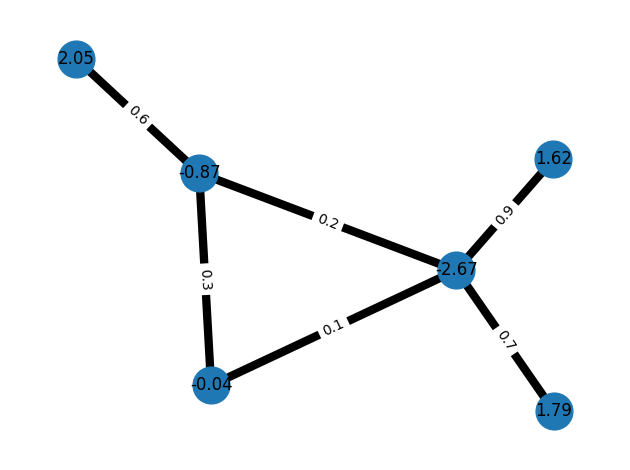
\includegraphics[width=0.45\textwidth]{figures/toy_graph_conv_K2.png}
        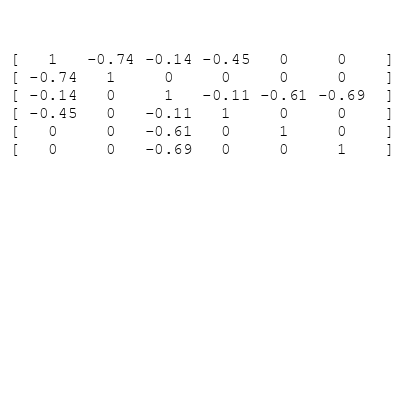
\includegraphics[width=0.45\textwidth]{figures/lap1.png}
        \caption{$\leftarrow$ After convolution with $K=2$ | $\tilde{L}$ $\rightarrow$}
    \end{subfigure}
    \hfill
    \begin{subfigure}{0.45\textwidth}
        \centering
        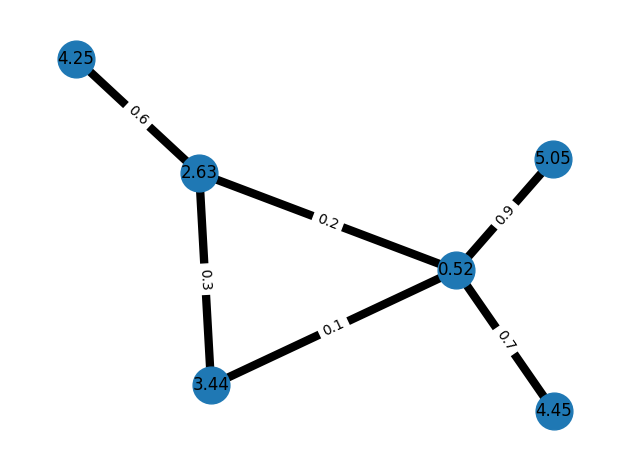
\includegraphics[width=0.45\textwidth]{figures/toy_graph_conv_K3.png}
        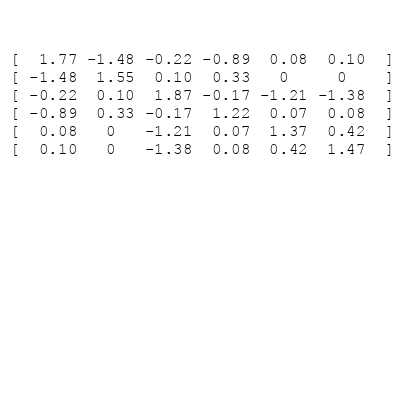
\includegraphics[width=0.45\textwidth]{figures/lap2.png}
        \caption{Convolution with $K=3$ | $\tilde{L}^2$ $\rightarrow$ }
    \end{subfigure}
    \caption{Convolution of a toy graph and the normalized Laplacian matrix $\widetilde{\mathbf{L}}^K$ for $K=1, 2, 3$.}
    \label{fig:toyGraph}
    \Description[]{illustration of convolution on graph}
 \end{figure}
For the example displayed in figure \ref{fig:toyGraph}, we initialized the weight of the convolution to one.



\section{Experiments}

\subsection{Proposed Modifications}
We studied various aspects of the methodology, including:
\begin{enumerate}
    \item The relevance of dimensionality reduction applied to features before training the neural networks.
    \item The approach of choosing a graph-based classification approach rather than a simple dense network operating on the vectorized feature vectors.
\end{enumerate}
As a result, we explored different techniques for dimensionality reduction and various classification models. We run the following experiments to address these questions.

Initially, we trained the models using the original features without any dimensionality reduction (1). Subsequently, we trained them with a reduced number of features achieved through recursive feature elimination (2), mirroring the approach detailed in the referenced paper. Finally, we applied an autoencoder to reduce feature dimensionality (3).

We implemented three distinct models:
\begin{enumerate}
    \item A simple Dense Neural Network consisting of linear layers and ReLU activations.
    \item A Graph Convolutional Network (GCN) as outlined in \cite{kipf_semi-supervised_2017}, incorporating the \textit{renormalization trick}.
    \item A neural network utilizing Chebyshev polynomials with an order of $K=3$, in accordance with the methodology presented in the referenced paper \cite{Parisot17}.
\end{enumerate}


\subsection{Dimensionality reduction by Recursive Feature Selection with a Ridge classifier}

A Ridge classifier is a standard linear classifier with an added regularization term known as the Ridge (L2) penalty.

The optimization problem of the ridge classifier is to find the coefficients $\beta$ that minimize the following objective function:
$$
\min_{\beta} \norm{y - X\beta}_2^2 + \alpha \norm{\beta}_2^2
$$
where $X$ is the design matrix, here the vectorized connectivity matrix, $y$ is the corresponding target value, $\alpha$ is the regularization parameter, and $\norm{.}_2$ denotes the Euclidean norm. The ridge classifier converts the targets values into $\{-1, 1\}$ and then treats the problem as a regression task. The predicted class corresponds to the sign of the regressor's prediction, which is
$$
\hat{y} = sign(X\hat{\beta})
$$
where $sign$ is a function that return $1$ if the input is positive, $-1$ if the input is negative, and $0$ if the input is zero.
% The Ridge penalty term, $\alpha \lVert w \rVert_2^2$, penalizes large values of the weights, encouraging a more generalizable model and helping to mitigate overfitting.

The recursive feature elimination (RFE) is employed to iteratively select features by progressively considering smaller sets of features. Initially, the estimator is trained on the complete set of features, and the importance of each feature $i$ is determined by evaluating the weights assigned to the Ridge estimator $\hat{\beta}_i$. Subsequently, the least important features are pruned from the current set and this process is repeated recursively on the pruned set until the desired number of features to select is reached.
\begin{figure*}[t!]
    \centering
    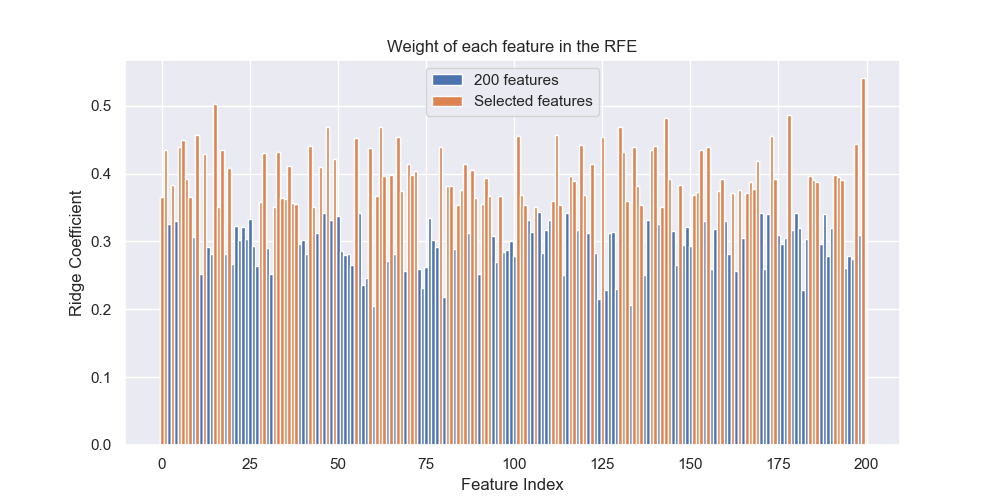
\includegraphics[width=0.8\textwidth]{figures/rfe.png}
    \caption{Relative importance of features for recursive elimination}
    \label{fig:rfe}
    \Description{}
\end{figure*}

\subsection{Dimensionality reduction by Autoencoder}



\section{Results and Discussion}



\subsection{Experimental setting}
In order to compare several methods (architecture, feature selection), we train on the ABIDE dataset with the systematic method of cross-validation proposed below.
\begin{itemize}
	\item We create 10 splits of the dataset with fixed seeds. Seeds are the same across all experiments.
	\item Each split is made of a training (80\%), validation (10\%) and test set (10\%).
	\item At training time, the whole population is present in the graph but only a fraction of the nodes are labeled (the 80\% of the training set).
	\item For each experiment configuration, we train 10 times the model with each split.
	We pick the epoch which corresponds to the minimum validation loss and take the corresponding test accuracy at this specific epoch. Mean and standard deviation of the accuracy across all splits.
\end{itemize}

We abbreviate the tested configurations as follows:
\begin{itemize}
	\item Single-h=$h$ refers to a single hidden layer with around 6000 features or 2000 when reduced, $h$ hidden neurons and a single output for binary classification.
	\item Dense refers to a fully connected neural network with 2 hidden layers and a final linear classifier.
	\item Cheb-dr=$dr$ refers to the Chebyshev spectral graph convolutional \cite{Defferrard2016} architecture with a dropout rate of $dr$.
\end{itemize}

We systematically used the Adam optimizer with a learning rate of $10^{-4}$ and a weight decay of $0.1$ and train for 1000 epochs.
The majority of models overfit the training dataset.
In all following boxplots, we report the original paper's accuracy (69.5\%) with a dashed purple line.

\subsection{Results on using reduced features}

In line with the methodology outlined in the original paper, we systematically selected a subset of $2000$ features with the RFE algorithm trained on a subset of 300 samples.

\begin{figure}[h!]
    \centering
    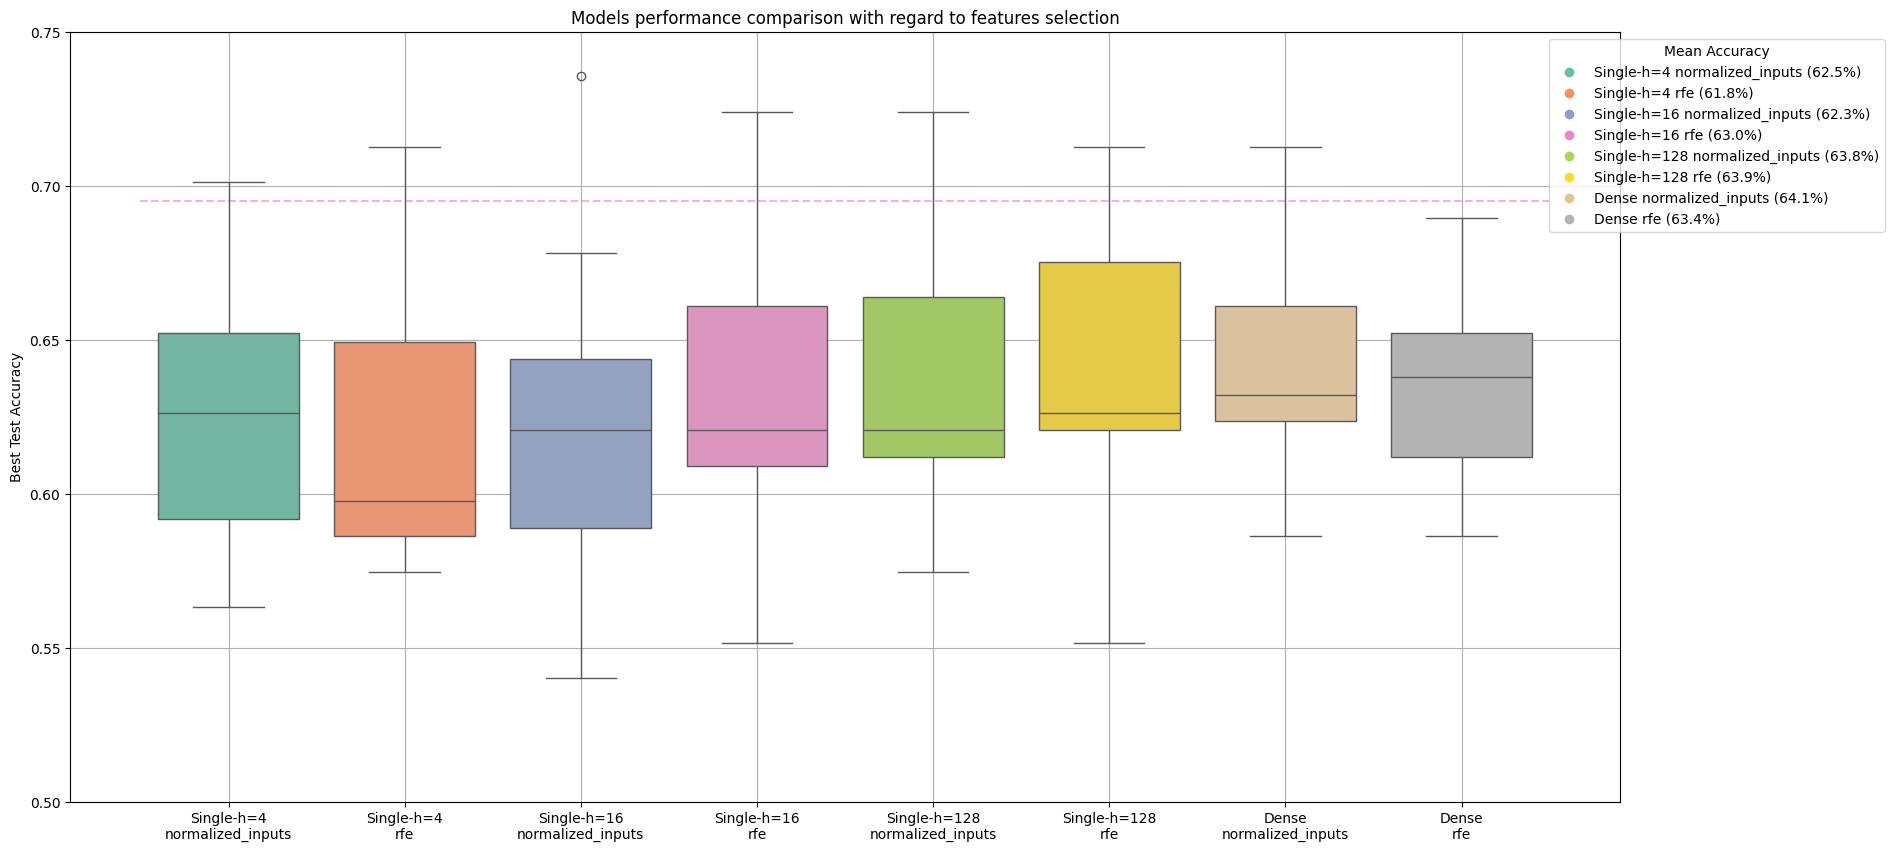
\includegraphics[width=0.5\textwidth]{figures/performances_fully_connected_RFE.png}
    \caption{No significant differences in performance between using all features and using a subset of 2000 features selected with RFE, no matter the number of neurons in the hidden layer.}
    \Description{}
    \label{fig:results_feature_reduction}
\end{figure}

\begin{table}[h!]
	\begin{center}
        \begin{tabular}{lll}
            Model & Feature & Test accuracy \\
            \hline
            Single-h=4 & normalized inputs & 62.5 +/- 4.2\% \\
            Single-h=4 & rfe & 61.8 +/- 4.4\% \\
            Single-h=4 & ae & 59.8 +/- 8.6\% \\
            Single-h=16 & normalized inputs & 62.3 +/- 5.4\% \\
            Single-h=16 & rfe & 63.0 +/- 5.1\% \\
            Single-h=16 & ae & 60.3 +/- 3.9\% \\
            Single-h=128 & normalized inputs & 63.8 +/- 4.3\% \\
            Single-h=128 & rfe & 63.9 +/- 4.6\% \\
            Single-h=128 & ae & 61.7 +/- 4.8\% \\
            Dense & normalized inputs & 64.1 +/- 3.4\% \\
            Dense & rfe & 63.4 +/- 3.3\% \\
            Dense & ae & 60.7 +/- 4.0\% \\
        \end{tabular}
    \end{center}
    \caption{Models performances with regard to feature reduction method.
	There is no obvious advantage to using a feature reduction method.}
    \label{table:dependance_on_feature_extraction_method}
\end{table}

Despite the varied configurations tested, it is notable that these setups did not result in significant differences in performance on the test data. Furthermore, the reduction of features through Recursive Feature Elimination (RFE) did not demonstrate any discernible improvement in performance.
Table \ref{table:dependance_on_feature_extraction_method} summarizes the results of our experiments on feature dimensionality reduction.

\subsection{Effect of using graph convolution}

The boxplot \ref{fig:results_architecture} displays the performance of the various configurations in our study. We observe that the use of graph convolutional layers improves the performance of the model as claimed by the authors of the original paper. All average performances
are reported in \ref{table:dependance_on_architecture}.

\begin{figure}[h!]
    \centering
    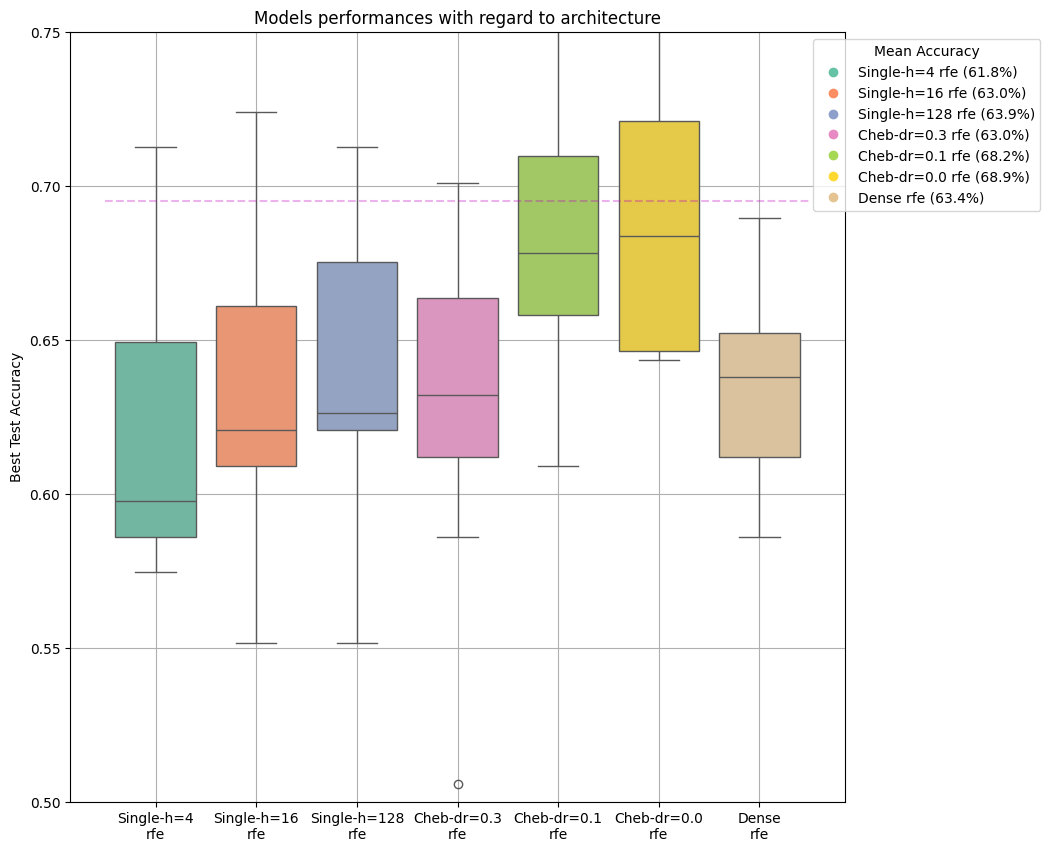
\includegraphics[width=0.45\textwidth]{figures/model_performances_architecture.png}
    \caption{Classification accuracy: comparison of different architectures.
    Single architectures are composed of a single hidden layer with a given number of neurons $h$.
    \textit{Dense} architecture refer to a fully connected neural network with a single hidden layer.
    \textit{Cheb} architectures refer to the graph convolution architecture, we vary the dropout rate $dr$
    during training.}
    \Description{}
    \label{fig:results_architecture}
\end{figure}

\begin{table}[H]
	\begin{center}
		\begin{tabular}{lll}
			Model & Feature & Test accuracy \\
			\hline
			Single-h=4 & rfe & 61.8 +/- 4.4\% \\
			Single-h=16 & rfe & 63.0 +/- 5.1\% \\
			Single-h=128 & rfe & 63.9 +/- 4.6\% \\
			Cheb-dr=0.3 & rfe & 63.0 +/- 5.4\% \\
			Cheb-dr=0.1 & rfe & 68.2 +/- 4.0\% \\
			Cheb-dr=0.0 & rfe & 68.9 +/- 4.0\% \\
			Dense & rfe & 63.4 +/- 3.3\% \\
		\end{tabular}
	\end{center}
	\caption{Models performances with regard to architecture}
	\label{table:dependance_on_architecture}
\end{table}




\section{Main limitations and conclusion}


One prominent challenge that emerged from our experiments was the significant discrepancy between the number of subjects ($871$) and the number of features (higher than $6100$), even after dimension reduction techniques were applied. This scenario places us squarely in the realm of the "curse of dimensionality," introducing complexities that can adversely impact the training of neural network models. With a limited number of subjects, the data points within the high-dimensional feature space become sparsely distributed. This sparsity poses challenges for neural networks, as they may struggle to capture meaningful patterns and relationships in the data, leading to overfitting or suboptimal generalization.

In particular, all the models were overfitting the training data, as evidenced by the large gap between the training (100\% accuracy) and validation accuracies (65\%). Despite our attempts to mitigate this issue (by applying dropout and $L_2$ regularization), neural network models always end up overfitting the training dataset. No matter how high the training accuracy gets, validation accuracy keeps increasing and we observe no degradation in the performances. This could be an instance of benign overfitting \cite{Bartlett_2020}. We note that the ChebGCN trained without dropout yields the best performance on the validation data 68.9 +/- 4.0\%, still not reaching the 69.5\% accuracy
mentioned in the original paper.


In conclusion, our experiments encompassed a range of configurations, each designed to explore different aspects of the model. Despite the diversity in hyperparameters and settings, the performance across these configurations on the test data exhibited minimal variations.



\bibliographystyle{ACM-Reference-Format}
\bibliography{references}

\end{document}
\endinput
%%
%% End of file `sample-sigconf.tex'.
